\setcounter{equation}{0}

\chapter{Introduction}

Inspired by the Kolmogorov-Arnold representation theorem (KART), Kolmogorov-Arnold Networks (KANs) provide a promising alternative to Multi-Layer Perceptrons (MLPs). KART states that any continuous, multi-variate function can be represented as a composition of univariate functions. While MLPs are inspired by the universal approximation theorem, KANs are inspired by KART. Like MLPs, KANs have fully-connected structures. However, KANs differ significantly from MLPs in how they handle activation functions:

MLPs apply fixed, non-linear activation functions to nodes, while KANs utilize learnable activation functions on edges. This seemingly minor change has profound implications for both accuracy and interpretability. KANs have no linear weight matrices at all. Instead, each weight parameter is replaced by a learnable univariate function, typically parameterized as a B-spline curve. KAN nodes simply sum incoming signals without applying non-linearities.

The theory behind KANs is KART (Kolmogorov-Arnold Representation Theorem). It underpins the theoretical foundation of KANs, enabling the decomposition of high-dimensional functions into compositions of lower-dimensional functions. This decomposition offers potential advantages in mitigating the curse of dimensionality, which often plagues traditional function approximation methods.
Neural Scaling Laws: KANs exhibit favorable scaling laws compared to MLPs, meaning their test loss decreases more rapidly as model size increases. The use of splines contributes to this superior scaling behavior by enabling accurate approximation of univariate functions within the network

\clearpage

\section{Background}

Kolmogorov-Arnold Networks (KANs) are a relatively new type of deep learning architecture inspired by the Kolmogorov-Arnold representation theorem (KART). This theorem, a fundamental result in approximation theory, posits that any continuous, multivariate function can be represented as a composition of univariate functions and addition operations. Building on this principle, KANs distinguish themselves from the more traditional Multi-Layer Perceptrons (MLPs) by shifting the location and nature of activation functions.

\begin{figure}[t]
    \centering
    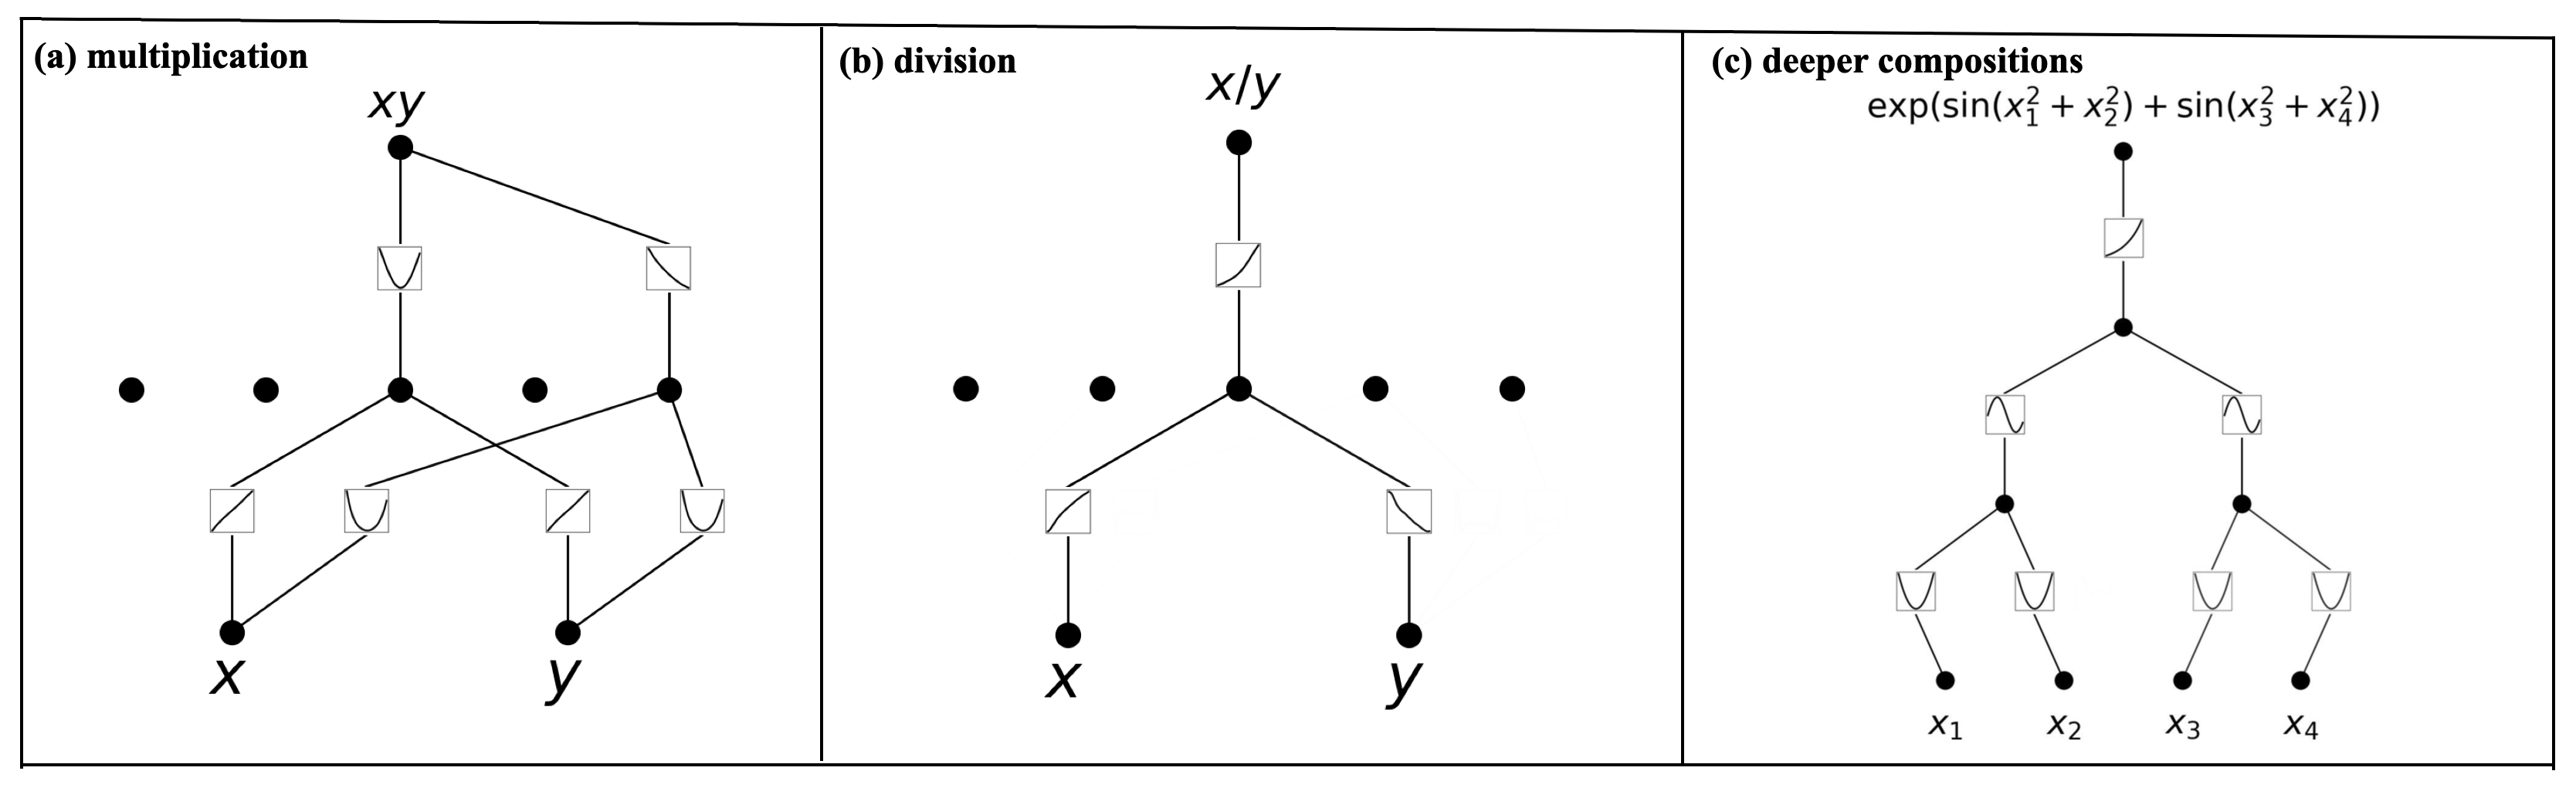
\includegraphics[width=0.9\linewidth]{Images/interpretable_examples_short.png}
    \caption{Interpretable examples of Kolmogorov-Arnold Networks (KANs) on synthetic tasks.}
    \label{fig:interpretable-examples}
\end{figure}

While MLPs have fixed, non-linear activation functions applied at nodes, KANs feature learnable activation functions positioned on the edges connecting the nodes. This key architectural difference has significant implications for both model accuracy and interpretability.
\begin{itemize}
    \item Eliminating Linear Weights: In a KAN, each edge houses a univariate function, typically parameterized using splines, effectively replacing the linear weight parameters found in MLPs. The nodes in a KAN perform simple summation of the incoming signals, devoid of any non-linear transformation.
    \item Spline Parameterization: The use of splines, piecewise polynomial functions, to represent the activation functions on edges offers several advantages. Splines are known for their accuracy in approximating low-dimensional functions and their ability to adjust locally, switching between different resolutions as needed. This makes them well-suited for capturing the nuances of univariate functions within the KAN framework.
\end{itemize}

\section{Motivation}

The development of KANs is driven by two primary objectives: enhancing accuracy and improving interpretability in deep learning models.

\begin{itemize}
    \item Combating the Curse of Dimensionality: Traditional approaches to function approximation often struggle with the "curse of dimensionality," where the complexity grows exponentially with the number of input variables. KANs, by leveraging the compositional structure inherent in KART, aim to mitigate this curse. By decomposing a high-dimensional function into a series of lower-dimensional functions, KANs can achieve better scaling laws compared to MLPs, particularly when the underlying function exhibits a compositional form.
    \item Enhanced Feature Learning: The combination of MLP-like external structure and spline-based internal mechanisms allows KANs to excel at both learning compositional structures and optimizing the learned features. KANs can, in a sense, learn both the "external degrees of freedom" (the relationships between variables) and the "internal degrees of freedom" (the precise form of the univariate functions).
    \item Visualization of Relationships: The structure of KANs, where activation functions are represented as 1D curves on edges, lends itself well to visual interpretation. By examining the shape and magnitude of these curves, one can gain insights into the relationships between input variables and their contribution to the output.
    \item Extracting Symbolic Formulas: Techniques like sparsification and pruning can be applied to KANs to simplify their structure and make them even more interpretable. In certain cases, it is possible to extract symbolic formulas from trained KANs, revealing the underlying mathematical relationships captured by the model. This capacity for symbolic regression makes KANs particularly appealing for scientific applications, where understanding the mathematical form of relationships is crucial.
\end{itemize}